\documentclass[12pt]{article}
\usepackage{amsthm,amssymb,amsfonts,amsmath,amstext,systeme}
\usepackage{graphicx,float}
\usepackage{tabularx}
\marginparwidth 0pt
\oddsidemargin -1.2 truecm
\evensidemargin  0pt 
\marginparsep 0pt
\topmargin -2.2truecm
\linespread{1}
\textheight 25.8 truecm
\textwidth 18.5 truecm
\newenvironment{remark}{\noindent{\bf Remark }}{\vspace{0mm}}
\newenvironment{remarks}{\noindent{\bf Remarks }}{\vspace{0mm}}
\newenvironment{question}{\noindent{\bf Question }}{\vspace{0mm}}
\newenvironment{questions}{\noindent{\bf Questions }}{\vspace{0mm}}
\newenvironment{note}{\noindent{\bf Note }}{\vspace{0mm}}
\newenvironment{summary}{\noindent{\bf Summary }}{\vspace{0mm}}
\newenvironment{back}{\noindent{\bf Background}}{\vspace{0mm}}
\newenvironment{conclude}{\noindent{\bf Conclusion}}{\vspace{0mm}}
\newenvironment{concludes}{\noindent{\bf Conclusions}}{\vspace{0mm}}
\newenvironment{dill}{\noindent{\bf Description of Dill's model}}{\vspace{0mm}}
\newenvironment{maths}{\noindent{\bf Mathematics needed}}{\vspace{0mm}}
\newenvironment{inst}{\noindent{\bf Instructions}}{\vspace{0mm}}
\newenvironment{notes}{\noindent{\bf Notes }}{\vspace{0mm}}
\newenvironment{theorem}{\noindent{\bf Theorem }}{\vspace{0mm}}
\newenvironment{example}{\noindent{\bf Example }}{\vspace{0mm}}
\newenvironment{examples}{\noindent{\bf Examples }}{\vspace{0mm}}
\newenvironment{topics}{\noindent{\bf Topics}}{\vspace{0mm}}
\newenvironment{outcomes}{\noindent{\bf Expected Learning Outcomes}}{\vspace{0mm}}
\newenvironment{lemma}{\noindent{\bf Lemma }}{\vspace{0mm}}
\newenvironment{solution}{\noindent{\it Solution}}{\vspace{2mm}}
\newcommand{\ds}{\displaystyle}
\newcommand{\un}{\underline}
\newcommand{\bs}{\boldsymbol}

\begin{document}

\baselineskip 18 pt
\begin{center}
	{\large \bf HKDSE MATH Core Sample Paper I}\\
	\vspace{2 mm}
\end{center}
\vspace{0.05cm}

\begin{enumerate}
	\item \textbf{HKDSE MATH Core Sample Paper I Q1}\\
	Simplify $\dfrac{(xy)^2}{x^{-5}y^6}$ and express your answer with positive indices. \\(3marks)

	\item \textbf{HKDSE MATH Core Sample Paper I Q2}\\
	Make $b$ the subject of the formula $a(b+7) = a+b$. \\(3 marks)

	\item \textbf{HKDSE MATH Core Sample Paper I Q3}\\
	Factorize 
	\begin{enumerate}
		\item[(a)] $3m^2-mn-2n^2$,
		\item[(b)] $3m^2-mn-2n^2-m+n$.
	\end{enumerate}
	(3 marks)

	\item \textbf{HKDSE MATH Core Sample Paper I Q4}\\
	The marked price of a handbag is \$560. It is  given that the marked price of the handbag is 40\% higher than the cost.
	\begin{enumerate}
		\item[(a)] Find the cost of the handbag.
		\item[(b)] If the handbag is sold at \$460, find the percentage profit.
	\end{enumerate}
	(4 marks)

	\item \textbf{HKDSE MATH Core Sample Paper I Q5}\\
	In a football league, each team gains 3 points for a win, 1 point for a draw and 0 point for a loss. The champion of the league plays 36 games and gains a total of 84 points. Given that the champion does not lose any games, find the number of games that the champion wins. \\(4 marks)
	
	\item \textbf{HKDSE MATH Core Sample Paper I Q6}\\
	Figure 1 shows a solid consisting of a hemisphere of radius $r$ cm joined to the bottom of a right circular cone of height 12 cm and base radius $r$ cm. It is given that the volume of the circular cone is twice the volume of the hemisphere.
	\begin{figure}[H]
		\centering
		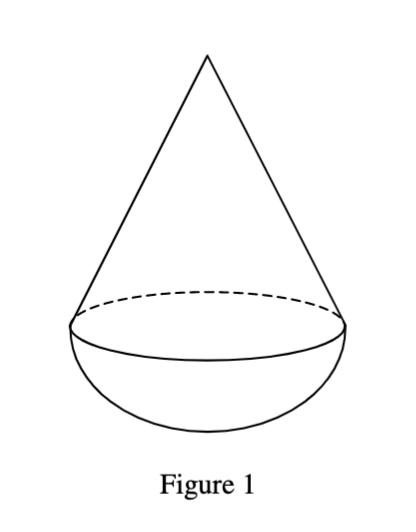
\includegraphics[width = .5\linewidth]{SPFigure1.1}
	\end{figure}
	\begin{enumerate}
		\item[(a)] Find $r$.
		\item[(b)] Express the volume of the solid in terms of $\pi$.
	\end{enumerate}
	(4 marks)

	\item \textbf{HKDSE MATH Core Sample Paper I Q7}\\
	In Figure 2, $O$ is the centre of the semicircle $ABCD$. If $AB//OC$ and $\angle BAD = 38^\circ$, find $\angle BDC$. \\(4 marks)
	\begin{figure}[H]
		\centering
		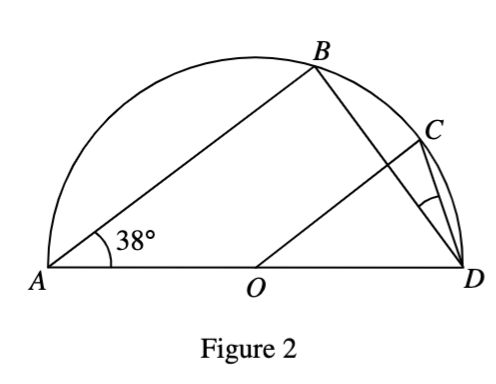
\includegraphics[width = .5\linewidth]{SPFigure1.2}
	\end{figure}

	\item \textbf{HKDSE MATH Core Sample Paper I Q8}\\
	In Figure 3, the coordinates of the point $A$ are $(-2, 5)$. $A$ is rotated clockwise about the origin $O$ through $90^\circ$ to $A'$. $A''$ is the refleciton image of $A$ with respect to the $y$-axis.
	\begin{figure}[H]
		\centering
		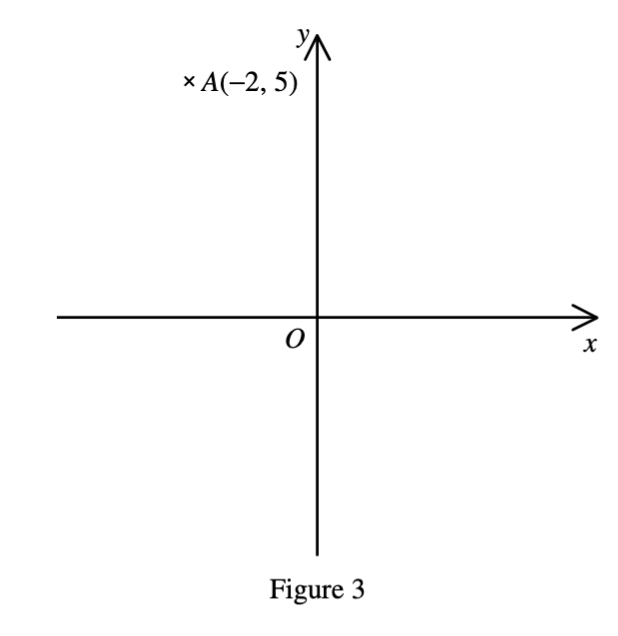
\includegraphics[width = .5\linewidth]{SPFigure1.3}
	\end{figure}
	\begin{enumerate}
		\item[(a)] Write down the coordinates of $A'$ and $A''$.
		\item[(b)] Is $OA''$ perpendicular to $AA'$? Explain your answer. 
	\end{enumerate}
	(5 marks)

	\item \textbf{HKDSE MATH Core Sample Paper I Q9}\\
	In Figure 4, the pie chart shows the distribution of the numbers of trafiic accidents occurred in a city in a year. In that year, the number of traffic accidents occurred in District A is 20\% greater than that in District B.
	\begin{figure}[H]
		\centering
		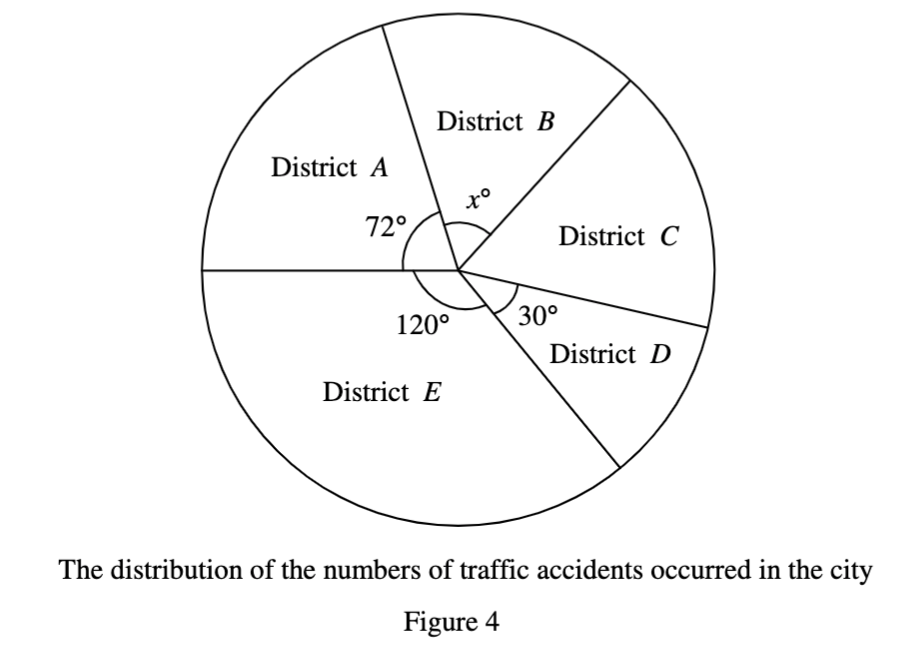
\includegraphics[width = .5\linewidth]{SPFigure1.4}
	\end{figure}
	\begin{enumerate}
		\item[(a)] Find $x$.
		\item[(b)] Is the number of traffic accidents occurred in District A grater than that in District C? Explain your answer. 
	\end{enumerate}
	(5 marks)
	

	\item \textbf{HKDSE MATH Core Sample Paper I Q10}
	\begin{enumerate}
		\item[(a)] Find the quotient when $5x^3 + 12x^2 - 9x - 7$ is divided by $x^2+2x-3$. \\(2 marks)
		\item[(b)] Let $g(x) = (5x^3 + 12x^2 - 9x - 7) - (ax+b)$, where $a$ and $b$ are constants. It is given that $g(x)$ is divisible by $x^2+2x-3$.
		\begin{enumerate}
			\item[(i)] Write down the values of $a$ and $b$.
			\item[(ii)] Solve the equation $g(x) = 0$.
		\end{enumerate}
		(4 marks)
	\end{enumerate} 

	\item \textbf{HKDSE MATH Core Sample Paper I Q11}\\
	In a factory, the production cost of a carpet of perimeter $s$ metres in \$ $C$. It is given that $C$ is a sum of two parts, one part varies as $s$ and the other part varies as the square of $s$. When $s = 2$, $C = 356$; when $s = 5$, $C = 1\,250$.
	\begin{enumerate}
		\item[(a)] Find the production cost of a carpet of perimeter 6 metres. \\(4 marks)
		\item[(b)] If the production cost of a carpet is \$539, find the perimeter of the carpet. \\(2 marks)
	\end{enumerate}

	\item \textbf{HKDSE MATH Core Sample Paper I Q12}\\
	Figure 5 shouws the graph for John driving from town $A$ to town $D$ (via town $B$ and town $C$) in a morning. The journey is divided into three parts: Part I(from $A$ to $B$), Part II(from $B$ to $C$) and part III(from $C$ to $D$).
	\begin{figure}[H]
		\centering
		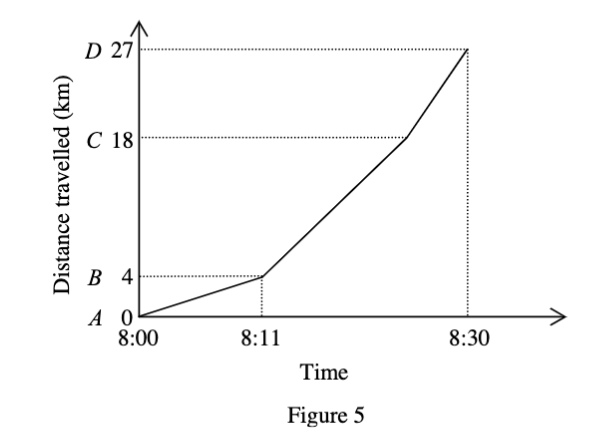
\includegraphics[width = .5\linewidth]{SPFigure1.5}
	\end{figure}
	\begin{enumerate}
		\item[(a)] For which part of the journey is the average speed the lowest? Explain your answer. \\(2 marks)
		\item[(b)] If the average speed for Part II of the journey is 56 km/h, when is John at $C$? \\(2 marks)
		\item[(c)] Find the average speed for John driving from $A$ to $D$ in m/s. \\(3 marks)
	\end{enumerate}

	\item \textbf{HKDSE MATH Core Sample Paper I Q13}\\
	In Figure 6, the straight line $L_1:4x-3y+12=0$ and the straight line $L_2$ are perpendicular to each other and intersect at $A$. It is given that $L_1$ cuts the $y$-axis at $B$ and $L_2$ passes through the point $(4,9)$.
	\begin{figure}[H]
		\centering
		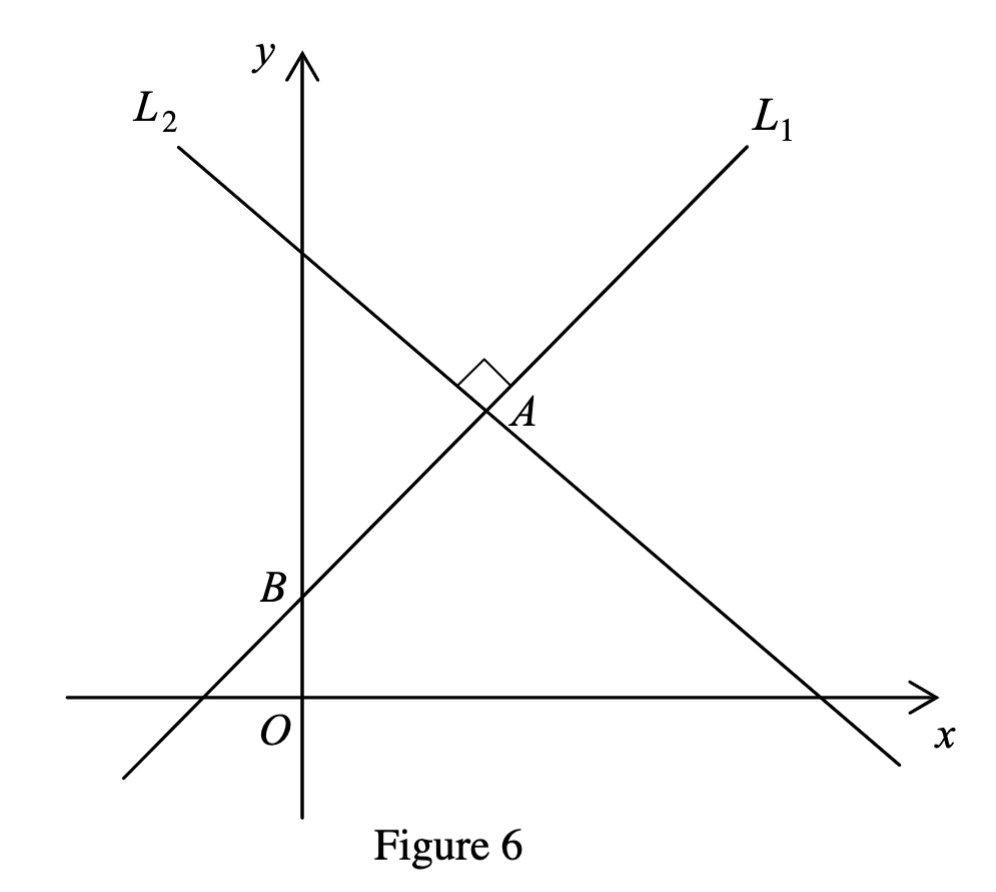
\includegraphics[width = .5\linewidth]{SPFigure1.6}
	\end{figure}
	\begin{enumerate}
		\item[(a)] Find the equation of $L_2$. \\(3 marks)
		\item[(b)] $Q$ is a moving point in the coordinate plane such that $AQ = BQ$. Denote the locus of $Q$ by $\Gamma$.
		\begin{enumerate}
			\item[(i)] Describe the geometric relationship between $\Gamma$ and $L_2$. Explain your answer.
			\item[(ii)] Find the equation of $\Gamma$.
		\end{enumerate}
		(6 marks)
	\end{enumerate}

	\item \textbf{HKDSE MATH Core Sample Paper I Q14}\\
	The data below show the percentages of customers who bought newspaper $A$ from a magazine stall in city $H$ for five days randomly selected in a certain week:
	$$62\% \quad 63\% \quad 55\% \quad 62\% \quad 58\%$$
	\begin{enumerate}
		\item[(a)] Find the meaidan and the mean of the above data. \\(2 marks)
		\item[(b)] Let $a\%$ and $b\%$ be the percentages of customers who bought newspaper $A$ from the stall for the other two days in that week. The two percentages are combined with the above data to form a set of seven data.
		\begin{enumerate}
			\item[(i)] Write down the least possible value of the median of the combnined set of seven data.
			\item[(ii)] It is known that the median and the mean of the combined set of seven data are the same as that found in (a). Write down one pair of possible values of $a$ and $b$.
		\end{enumerate}
		(3 marks)
		\item[(c)] The stall-keeper claims that since the median and the mean found in (a) exceed 50\% newspaper $A$ has the largest market share among the newspapers in city $H$. Do you agree? Explain your answer. \\(2 marks) 
	\end{enumerate}

	\item \textbf{HKDSE MATH Core Sample Paper I Q15}\\
	The seats in a theatre are numbered in numerical order from the first row to the last row, and from left to right, as shown in Figure 7. The first row has 12 seats. Each succeeding row has 3 more seats than the previous one. If the theatre cannot accommodate more than 930 seats, what is the greatest number of rows of seats in the theatre? \\(4 marks)
	\begin{figure}[H]
		\centering
		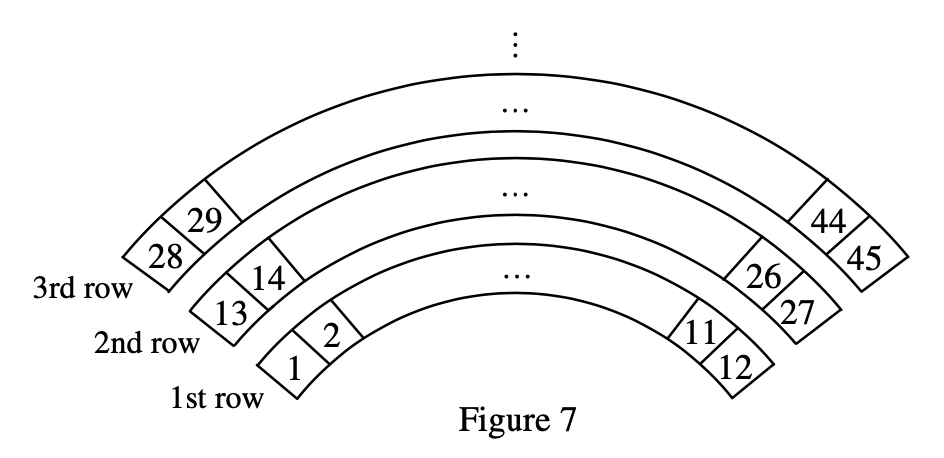
\includegraphics[width = .5\linewidth]{SPFigure1.7}
	\end{figure}

	\item \textbf{HKDSE MATH Core Sample Paper I Q16}\\
	A committee consists of 5 teachers from school $A$ and 4 teachers from school $B$. Four teachers are randomly selected from the committee.
	\begin{enumerate}
		\item[(a)] Find the probability that only 2 of the selected teachers are from school $A$. \\(3 marks)
		\item[(b)] Find the probability that the numbers of selected teachers from school $A$ and school $B$ are
		different. \\(2 marks)
	\end{enumerate}

	\item \textbf{HKDSE MATH Core Sample Paper I Q17}\\
	A researcher defined Scale $A$ and Scale $B$ to represent the magnitude of an explosion as shown in the following table:
	$$\begin{array}{|c|c|}
		\hline
		\text{Scale} & \text{Formula} \\
		\hline
		A & M = \log_4{E} \\
		\hline		
		B & N = \log_8{E} \\
		\hline
	\end{array}$$
	It is given that $M$ and $N$ are the magnitudes of an explosion on Scale $A$ and Scale $B$ respectively while $E$ is the relative energy released by the explosion. If the magnitude of an explosion is 6.4 on Scale $B$ , find the magnitude of the explosion on Scale $A$. \\(5 marks)

	\item \textbf{HKDSE MATH Core Sample Paper I Q18}\\
	In Figure 8(a), $ABC$ is a triangular paper card. $D$ is a point lying on $AB$ such that $CD$ is perpendicular to $AB$ . It is given that $AC = 20$ cm, $\angle CAD = 45^\circ$ and $\angle CBD = 30^\circ$.
	\begin{figure}[H]
		\centering
		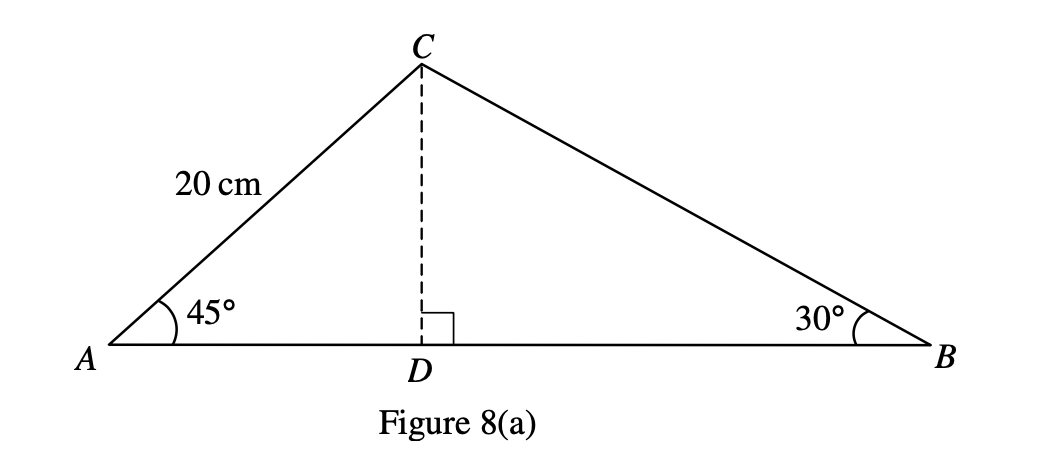
\includegraphics[width = .5\linewidth]{SPFigure1.8a}
	\end{figure}
	\begin{enumerate}
		\item[(a)] Find, in surd form, $BC$ and $BD$. \\(3 marks)
		\item[(b)] The triangular paper card in Figure 8(a) is folded along $CD$ such that $\triangle ACD$ lies on the horizontal plane as shown in Figure 8(b).
		\begin{figure}[H]
			\centering
			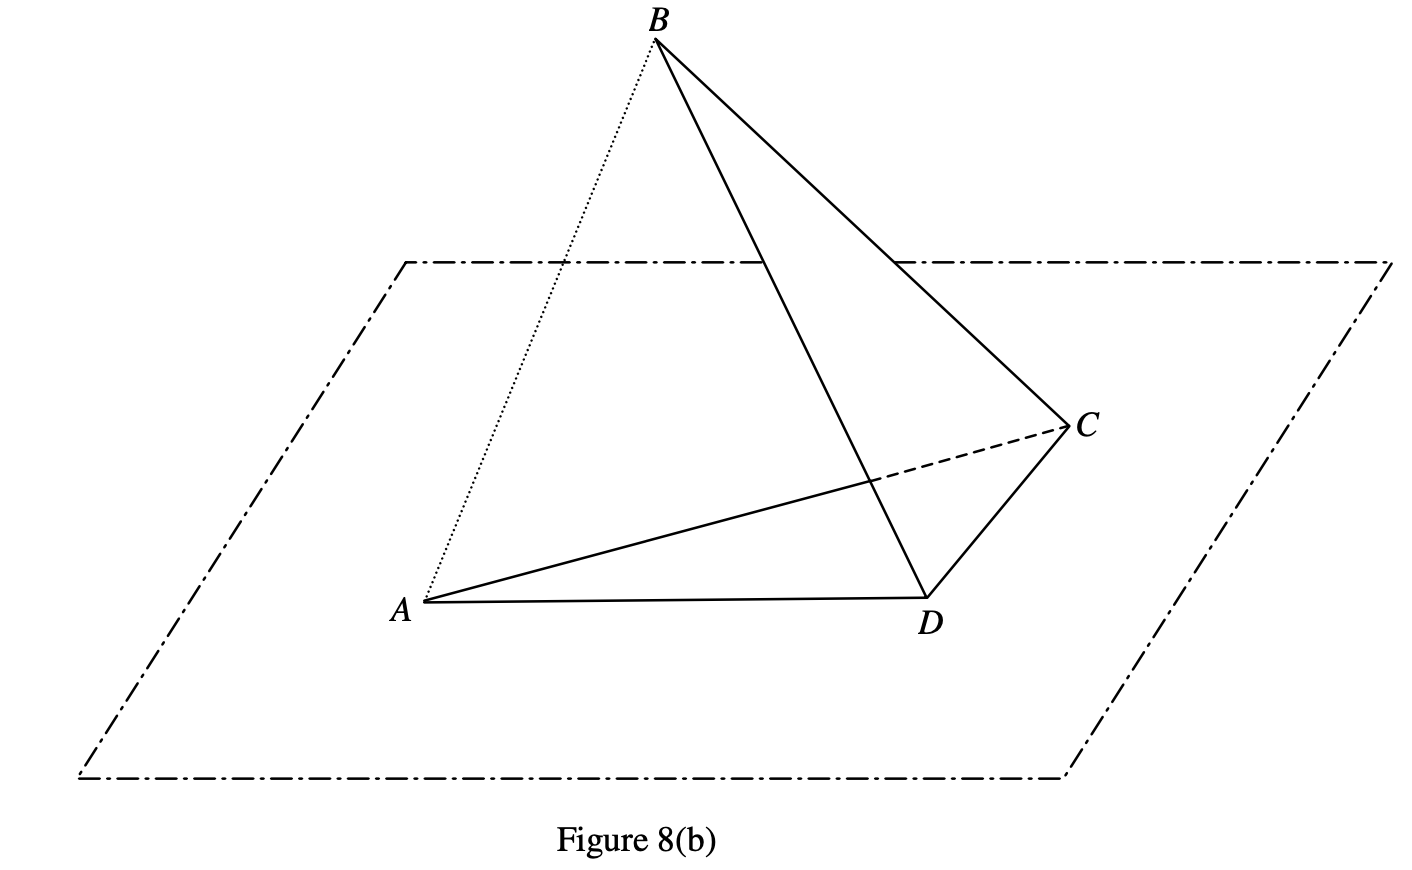
\includegraphics[width = .5\linewidth]{SPFigure1.8b}
		\end{figure}
		\begin{enumerate}
			\item[(i)] If the distance between $A$ and $B$ is 18 cm, find the angle between the plane $BCD$ and the horizontal plane.
			\item[(ii)] Describe how the volume of the tetrahedron $BCDA$ varies when $\angle ADB$ increases from $40^\circ$ to $140^\circ$. Explain your answer.
		\end{enumerate}
		(5 marks)
	\end{enumerate}

	\item \textbf{HKDSE MATH Core Sample Paper I Q19}\\
	In Figure 9, the circle passes through four points $A$, $B$, $C$ and $D$. $PQ$ is the tangent to the circle at $C$ and is parallel to $BD$. $AC$ and $BD$ intersect at $E$. It is given that $AB = AD$.
	\begin{figure}[H]
		\centering
		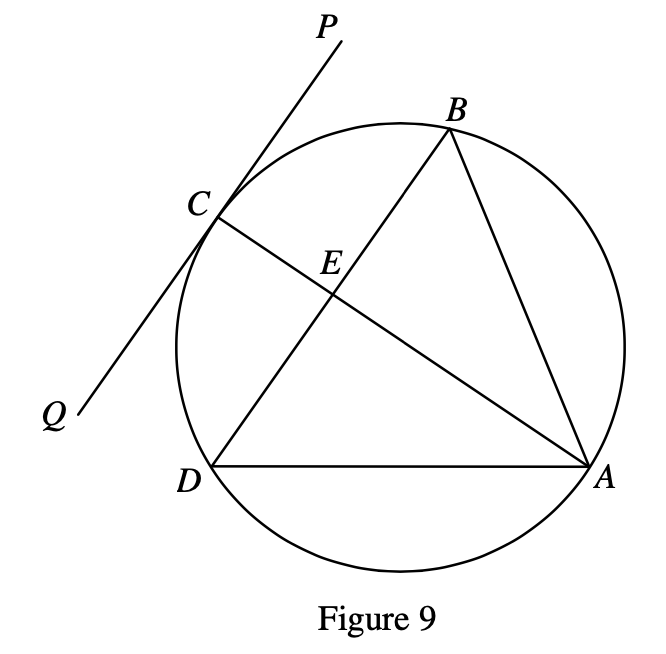
\includegraphics[width = .5\linewidth]{SPFigure1.9}
	\end{figure}
	\begin{enumerate}
		\item[(a)]
		\begin{enumerate}
			\item[(i)] Prove that $\triangle ABE \equiv \triangle ADE$.
			\item[(ii)] Are the in-centre, the orthocentre, the centroid and the circumcentre of $\triangle BDA$ collinear? Explain your answer.
		\end{enumerate}
		(6 marks)
		\item[(b)] A rectangular coordinate system is introduced in Figure 9 so that the coordinates of $A$, $B$ and $D$ are $(4,14)$, $(12,8)$ and $(4,4)$ respectively. Find the equation of the tangent $PQ$. \\(7 marks)
	\end{enumerate}
\end{enumerate}
\end{document}

